\section{Importance Sampling}
\label{sec:importance_sampling}
Importance sampling is a simulation technique that allows us to approximate integrals w.r.t a measure of interest, the target, by sampling from a tractable approximation, the proposal, instead, thus performing Monte-Carlo integration. To account for the fact that we did not sample from the correct probability measure, we weight samples according to their importance. As the user has freedom in the choice of approximation (except for some technical conditions), importance sampling also acts as a variance reduction technique with better approximations resulting in smaller Monte-Carlo variance. Thus the role that importance sampling plays is twofold: first, it enables Monte-Carlo integration even if sampling from the target is not possible, and second it allows us to do so in an efficient way by choosing, to be defined precisely below, the approximation in an optimal way.

Alternative approaches to importance sampling for performing inference in \glspl{ssm} include \gls{mcmc} and \gls{smc}. 
Recall from the introduction to this chapter that this inference concerns three objectives: maximum likelihood estimation, i.e. evaluation and optimization of the likelihood, access to the posterior distribution $X_{:n} | Y_{:n}$ and prediction of future states and observations. Let us give a concise comparison of these alternative approaches, weighing their advantages and disadvantages over importance sampling, in particular for the \glspl{ssm} that this thesis deals with. 

% MCMC intro
\gls{mcmc} \citep{Brooks2011Handbook} is a simulation technique that allows to simulation of correlated samples from a target distribution by constructing a Markov chain that has as its invariant distribution the desired distribution. For Metropolis-Hastings \gls{mcmc}, one needs access to the density of the sought distribution up to a constant to simulate a step in the Markov chain. While this method is very general, it fails in high dimensions and current research in \gls{mcmc} methods investigates this \todo{quotes} curse of dimensionality \todo{citep something}. 

% MCMC vs IS
\todo{MCMC vs. IS}

% SMC intro
\gls{smc} \citep{Chopin2020Introduction} or particle filters, use sequential importance sampling to provide a particle approximation to the filtering distributions $X_{t} | Y_{:t}$, essentially decomposing the problem into a $n$ importance sampling steps. 
To avoid particle collapse, \gls{smc} is usually equipped with a resampling step once the effective sample size of the current set of particles drops below a specified level. Once the final filtering distribution $X_{n}|Y_{:n}$ is approximated, the smoothing distribution may be obtained in several ways ... \todo{look up Chopin}.

% SMC vs. IS
Conveniently, \gls{smc} allows us to approximate the likelihood $\ell(\theta)$ for a single parameter by a single pass of the particle filter. However, the discrete nature of resampling makes the approximated likelihood non-continuous, complicating maximum likelihood inference. \citep[Chapter 14]{Chopin2020Introduction} discusses several strategies: the first amounts to importance sampling of the order as discussed in this thesis, where one fixes a reference parameter $\theta_{0}$ to perform importance sampling with $p_{\theta_{0}}(x|y)$ against $p_{\theta}(x|y)$. The second strategy only works in the univariate case and consists of approximating the non-continuous inverse CDFs appearing in the resampling step by continuous ones. Finally, if the dependence on the hyperparameters $\theta$ allows for application of the EM-algorithm, it may be used to perform the optimization. 
Contrary to \gls{smc}, the global importance sampling approach we discuss in \Cref{sec:gaussian_importance_sampling_for_state_space_models,sec:maximum_likelihood_estimation} allows us to perform \todo{...}

This chapter proceeds with a general treatment of importance sampling, loosely based on \citep[Chapter 8]{Chopin2020Introduction} and \citep[Chapter 11]{Durbin2012Time}. Subsequently, we will focus our attention on methods to obtain good importance sampling proposals. 

Suppose we have a function $h: \mathcal X \to \R$ whose integral w.r.t. to some measure $\mu$, $$\zeta = \int_{\mathcal X} h(x) \d\mu(x),$$ exists and whose value we want to compute. 
Furthermore, suppose that we can write
$$
    \int_{\mathcal X} h(x) \d \mu(x) = \int_{\mathcal X} f(x) \d \P(x) = \P [f],
$$
\todoTH{operatorschreibeweise everywehere}
for a probability measure $\P$ and function $f: \mathcal X \to \R$, e.g. because $\P = p \mu$ and $h(x) = f(x) p(x)$ $\mu$-a.s. .
Let $\G$ be a another probability measure on $\mathcal X$ such that $f\P$ is absolutely continuous with respect to $\G$, $f\P \ll \G$, and let $v = \frac{\d f\P}{\d\G}$ be the corresponding Radon-Nikodym derivative. Then
$$
    \zeta = \P [f] = \int_{\mathcal X} f(x) \d \P(x) = \int_{\mathcal X} \left(\rnd{f\P}{\G}\right)\d\G(x) = \G [v]
$$
which suggests to estimate $\zeta$ by Monte-Carlo integration: $$\hat \zeta = \frac 1 N \sum_{i=1}^{N} v(X^{i}), $$ the importance sampling estimate of $\zeta$. The importance samples $X^{i}, i = 1, \dots, N$ have distribution $\G$, and will usually be i.i.d.. For this procedure to work, we want $\hat \zeta$ to fulfill a law of large numbers and a central limit theorem, so we will want $v \in L^{2}(\G)$, where $L^{p}(\nu)$ is the space of $p$-times $\nu$-integrable functions for a measure $\nu$. The i.i.d. assumption could also be dropped, e.g. when we employ antithetic variables, see \citep[Section 5.3]{Ripley2009Stochastic}. Here we call $\hat \zeta$ the importance sampling estimate of $\zeta$. 

If $v \in L^{2}(\G)$ and under i.i.d. sampling the Monte-Carlo variance of $\hat \zeta$ is $\frac{\var \left(v(X^{i})\right)}{N}$, and so naturally we want $\var \left(v(X^{i})\right)$ to be small to ensure fast convergence of $\hat \zeta$. As $v$ depends on the proposal $\G$, and we have the flexibility to choose $\G$, importance sampling acts as a variance reduction technique. 

A classical result is that the minimum MSE proposal $\G^\ast$ has a closed form. Indeed it is given by the total variation measure of $f\P$, renormalized to be a probability measure, which can be shown by a simple application of Jensen's inequality. 
\begin{proposition}[{\cite[Proposition 8.2]{Chopin2020Introduction}}][minimum MSE proposal]
    \label{prop:minimum_MSE_IS}
    The proposal $\G^{\ast}$ that minimizes the MSE of importance sampling is given by
    $$
    \G^{\ast}  = \frac{\lvert f \rvert}{\P\left[\lvert f \rvert \right]} \P.
    $$
\end{proposition}
Unfortunately, this optimality result has no practical use, indeed if $f$ is positive we would need to obtain $\P[f]$ first, the overall target of our endeavor. Additionally, sampling from $\G^{\ast}$ is not guaranteed to be practically feasible. 

If the Radon-Nikodym derivative $w = \frac{\d\P}{\d\G}$ exists, then $v = fw$, which, for the problems we will study, is usually the case. In this case 
$$
\hat \zeta = \frac{1}{N} \sum_{i = 1}^N f(X^{i})w(X^{i}),
$$
where $w(X^{i})$ is called the importance weight, or just weight, of the $i$-th sample. If the samples is clear from the context we sometimes write $w^{i} = w(X^{i})$. 
This motivates us to regard
%If one is not interested in a particular function $f$, we may instead think of
\begin{align}
\label{eq:is-particle-approximation}
\hat \P_N = \frac{1}{N} \sum_{i = 1}^{N} w(X_i) \delta_{X_i},
\end{align}
as a particle approximation of $\P$, in the sense that for sufficiently well behaved test functions $f$, as $N \to \infty$ $$
\hat\P_{N}[f] = \frac{1}{N} \sum_{i = 1}^N f(X^{i})w(X^{i})\to \P [f].
$$
We will return to the question of which functions $f$ to consider further below and assume in the following discussion $fw \in L^{2}(\G)$.

To perform importance sampling one must be able to evaluate $w$. In the context of \acrshortpl{pgssm} this is usually not possible: if $\P$ is the intractable conditional distribution of $X|Y$, then the integration constant of its density $p(y)$ is not analytically available.
Still, we can usually evaluate the weights up to a constant, i.e. $$\tilde w(x) \propto \frac{\d \P}{\d \G}(x)$$ is available. The missing constant is then $\G \tilde w$, which is itself amenable to importance sampling: we may estimate it by $\sum_{i = 1}^N \tilde w(X^{i})$.
This leads to the so-called self-normalized importance sampling weights 
$$W_i = \frac{w(X^i)}{\sum_{i = 1}^N w(X^i)},$$
Monte Carlo estimates 
$$\hat \zeta = \sum_{i = 1}^{N} W_i f(X^i),$$
and particle approximation 
$$\hat \P_N = \sum_{i = 1}^{N} W_i \delta_{X^i}.$$

% introduces bias
Unless $\tilde w$ is degenerate, i.e. constant, $$\hat\zeta = \frac{\sum_{i = 1}^N \tilde w (X^{i} f(X^{i}))}{\sum_{i = 1}^{N} \tilde w(X^{i})}$$ is a ratio of two non-constant, unbiased estimators and so is itself biased. Nevertheless, noticing that the rescaled denominator $\frac{1}{N} \sum_{i = 1}^{N} \tilde w(X^{i})$ consistently estimates the integration constant $\G \tilde w$, allows us to apply Slutsky's lemma and obtain a central limit theorem for $\hat \zeta$ (recall that we assumed $fw \in L^{2}(\G)$).

% introduce probabilit metrics from Agapiou
The class for test functions $f$ for which this holds depends on $\P$ and $\G$. \citep{Agapiou2017Importance} study the behavior of uniformly bounded test functions $\lVert f \rVert \leq 1$. For these functions it suffices that $w \in L^{2}(\G)$ to ensure asymptotic normality of $\zeta$. 
%In this setting they show that the random measure $\hat \P_N$ converges to $\P$ at usual rate $\mathcal O\left(\frac 1 {\sqrt{N}}\right)$ in an appropriate metric on the space of random probability measures. 
Thus an important quantity is
$$
\rho = \frac{1}{(\G \tilde w)^{2}}\G[\tilde w^{2}] = \G [w^{2}] =  \P [w],
$$
the second moment of the importance sampling weights. \citep{Agapiou2017Importance} show that the bias 
$$
\left| \mathbb E (\hat\P_{N} - \P)[f] \right|
$$
and \acrfull{mse}
$$
\mathbb E \left( (\hat \P_{N} - \P) [f] \right)^{2}
$$
of importance sampling are both, for bounded $f$, of order $\mathcal O \left(\frac{\rho}{N}\right)$. Here the expectation $\mathbb E$ is with respect to the random particles $X^{1}, \dots, X^{N}$. Consequently, for bounded functions, keeping $ \frac{\rho}{N}$ small produces importance sampling estimates with small bias and \acrshort{mse}. This can be achieved in two ways: either we choose $\G$ \glqq{}close enough\grqq{} to $\P$ to ensure small $\rho$, or we choose $N$ large enough to compensate for a large $\rho$.

Applying Jensen's inequality, we see that
$$
\Dkl{\P}{\G} = \P [\log w] \leq \log \P[w] = \log\rho,
$$
so small $\rho$ implies a small \acrshort{kld} as well. Conversely, the following theorem of \citeauthor{Chatterjee2018Sample} implies that a small \acrshort{kld} is both sufficient and necessary for importance sampling to perform well.
\begin{theorem}[{\cite[Theorem 1.1]{Chatterjee2018Sample}}]
    \label{thm:chatterje2018Thm1}
     Let $\P$ and $\G$ be probability measures on a measurable space $(\mathcal X, \mathcal B)$ such that $\P \ll \G$ and let $f \in \mathbf L^2(\P)$ be a function with $\lVert f \rVert_{L^{2}(\P)} = \left( \P f^{2} \right)^{1 / 2} < 
     \infty$. Let $Z$ be an $\mathcal X$ valued random variable with law $\P$. 
     
     Let $L = \Dkl{\P}{\G} = \mathbb E \log w(Y)$ be the \acrshort{kld} between $\P$ and $\G$, and let $$\hat \P_N = \sum_{i = 1}^N w(X^i) \delta_{X^i}$$ be the particle approximations of $\P$  based on samples $X^1, \dots, X^N\iid \G$, $N \in \N$. 
     
     If the sample size $N$ is given by $N = \exp\left( L + t \right)$ for a $t \geq 0$,
     \begin{align} \label{eq:chatterje-upper-bound}\mathbb E \left\lvert \hat \P_N[f] - \P [f] \right\rvert \leq \lVert f \rVert^2_{L^2(\P)} \left(\exp(-t / 4) + 2 \sqrt{\mathbb P \left( \log w(Z) > L + t / 2 \right)}\right). \end{align}

    Conversely, if $N = \exp \left( L - s \right)$ for $s \geq 0$, then for any $\delta \in (0,1)$ 
    \begin{align}
        \label{eq:chatterje-lower-bound}
    \mathbb P (\hat \P_{N}[ \mathbf 1 ] \geq 1 - \delta) \leq \exp \left( -\frac{s}{2} \right) + \frac{\mathbb P \left( \log w(Z) \leq L -\frac{s}{2} \right)}{ 1- \delta},
    \end{align}
    where $\mathbf 1$ is the constant function $x \mapsto 1$.

     Notice the boldface $\mathbb P$ and $\mathbb E$ to differentiate the measures $\P$ and $\G$ from expectations and probabilities with respect to the abstract probability space $\left( \Omega, \mathcal A, \mathbb P \right)$ where the random variables $X_{1}, \dots, X_{N}$ and $Y$ live.
\end{theorem}

The proof of this theorem is based on splitting $\mathcal X$ into $\{\log w \leq L + \frac{t}{2}\} $ and its complement and straightforward, it may be found in the Appendix of \citep{Chatterjee2018Sample}. Theorem 1.2 in the same paper provides a qualitatively similar result for autonormalised importance sampling.

Let us consider the implications of \Cref{thm:chatterje2018Thm1}, starting with \Cref{eq:chatterje-upper-bound}, by devising heuristics to decide when $\G$ is a good proposal for fixed sample size $N$, and assume for simplicity that $ \lVert f \rVert^{2}_{L^{2}(\P)} = 1 $.
First of all, as $t = \log N - L$, we have $\exp(- t / 4) =  \frac{\exp (L / 4)}{N^{4}}$, so for large $N$ this term becomes negligible fast, and the interesting term in \Cref{eq:chatterje-upper-bound} is the second one. As $\E \log w(Z) = L$, this term is a tail probability and we can use standard mass-concentration inequalities to analyze its behavior as $t$ (and so $N$) grows. Markov's inequality tells us that 
$$
\mathbb P \left( \log w(Z) > L + \frac{t}{2} \right) \leq \frac{L}{L + t / 2} = \frac{2}{1 + \frac{\log N}{L}}.
$$

Second, if, additionally, $\log w(Z)$ has finite variance, Tchebyscheff's inequality yields 
$$
\mathbb P \left( \log w (Z) > L + \frac{t}{2} \right) \leq \frac{4\operatorname{Var} (\log w(Z))}{t^{2}} = \frac{4\operatorname{Var} (\log w(Z))}{\left( \log N - L \right)^2}.
$$

In both upper bounds provided by the concentration inequalities, all else being equal, a smaller \acrshort{kld} will yield a tighter bound. However, in Tchebyscheff's inequality, the variance of log weights also plays a role, and will surely be different for different proposals.
Assuming $\G \ll \P$, we have $ \frac{\d \G}{\d\P} = \frac{1}{w}$ and so 
$$\mathbb E \exp (- \log w(Z) ) = \mathbb E \frac{1}{w(Z)} = \P \left[\frac{\d \G}{\d\P}\right] = 1,$$
If the log-weights are bounded from above and below, the following lemma shows that as the variance of $U = -\log w(Z)$ goes to $0$, their mean,
$$
\mathbb E U = \mathbb E - \log w(Z) = -\Dkl{\P}{\G}
$$
goes to $0$ as well.
\begin{lemma}
    \label{lem:bounded-log-variance}
    For $a,b \in \R$, let $U \in [a,b]$ be a bounded random variable with variance $\sigma^{2}$ and $\mathbb E \exp U = 1$. Let $\mu = \E U$ be the mean of $U$. Then there exists a $\delta \in [a,b]$, such that 
    $$
    0 \geq \mu = \log \left( 1 - \delta \frac{\sigma^{2}}{2} \right).
    $$
    If, additionally, $\sigma^{2} < \frac{2}{b}$ then 
    $$
    \mu \geq \log \left( 1 - b \frac{\sigma^{2}}{2} \right).
    $$
\end{lemma}

\begin{proof}
    As $U$ is bounded, all involved expectations exist and are finite. That $\mu \leq 0$ follows from Jensen's inequality. We perform a first-order Taylor expansion of $\exp(U - \mu)$, where the random variable $\xi$ is between $U - \mu$ and $0$:
    $$
    1 = \exp(\mu)\mathbb E \exp (U - \mu) = \exp (\mu) \left( 1 + \mathbb E (U - \mu) + \mathbb E\left(\frac{(U-\mu)^{2}}{2} \exp(\xi)\right) \right).
    $$
    Then $\xi' = \xi + \mu \in [a,b]$. 
    Thus
    $$
    1 = \exp(\mu) + \mathbb E\left(\frac{(U-\mu)^{2}}{2} \exp(\xi')\right),
    $$
    and as $\xi' \in [a,b]$, the expectation is in $\left[\exp(a) \frac{\sigma^{2}}{2}, \exp(b) \frac{\sigma^{2}}{2}\right]$, i.e. $\mathbb E\left(\frac{(U-\mu)^{2}}{2} \exp(\xi')\right) = \delta \frac{\sigma^{2}}{2}$ for some $\delta \in [a,b]$. Solving for $\mu$, we get 
    $$
    \mu = \log \left( 1 - \delta \frac{\sigma^{2}}{2} \right),
    $$
    as promised.

    The second statement follows from $\delta \leq b$ and the monotonicity of $\log$, where the condition ensures that the argument is positive.
\end{proof}

\begin{corollary}
    Let $\P$ and $\G$ be equivalent probability measures with bounded Radon-Nikodym derivative $w = \frac{\d\P}{\d\G} \in [a,b]$, $a, b \in \R$, finite \acrshort{kld} $\Dkl{\P}{\G} =\P [\log w] < \infty$.
    
    If $\log w \in L^{2}(\P)$ with variance $\sigma^{2} = \P [(\log w - L)^2]$, and $\sigma^{2} < \frac{2}{b}$, then 
    $$
    \Dkl{\P}{\G} \leq - \log \left(1 - \exp(b) \frac{\sigma^{2}}{2} \right).
    $$
\end{corollary}
Under the assumptions of this corollary, we see that a small variance of the log-weights implies a small \acrshort{kld}, which in turn implies good importance sampling performance.

Let us now discuss the implications of \Cref{eq:chatterje-lower-bound}. We see that for large $s$, i.e. $N \ll \exp(L)$, the right-hand side is small, and so the probability that importance sampling fails for the constant function is practically relevant. Thus \citeauthor{Chatterjee2018Sample} recommend to choose $N = \mathcal O( \exp \left( \Dkl{\P}{\G} \right))$. 

Based on this discussion, we see that choosing $\G$ such that either the \acrshort{kld} or the variance of the log-weights is small is sensible. Making the variance small has the additional advantage that it, at least for bounded log-weights, also implies an upper bound for the \acrshort{kld}. We will return to this train of thought when we discuss optimal ways of performing importance sampling, such as the \acem (minimizing the \acrshort{kld}) and \aeis (minimizing the variance of log-weights) in the following sub-chapters.

In practice, we will want to judge whether for an actual sample $X^{1}, \dots X^{N} \iid \G$ importance sampling has converged, and there are several criteria available in the literature. The classic \gls{ess}\citep{Kong1994Sequential} 
$$
\text{ESS} = \frac{1}{\sum_{i = 1}^N W^{2}_{i}} \in \left[1, N\right]
$$
arises from an analysis of the asymptotic efficiency of importance sampling estimates: Consider additional $Y^{1}, \dots, Y^{N}\iid \P$, a test function $f \in L^{2} (\P)$ and assume that $\rho < \infty$. We may then estimate $\zeta = \P f$ in two ways: either by using the importance sampling estimate 
$$
\hat \zeta_{\text{IS}} = \hat \P_{N} (f) = \sum_{i = 1}^N W_{i} f(X^{i}) = \frac{1}{N} \sum_{i = 1}^N (NW_{i}) f(X^{i}),
$$
or by standard Monte-Carlo integration 
$$
\hat \zeta_{\text{MC}} = \frac{1}{N}\sum_{i = 1}^N f(Y^{i}).
$$
\citep{Kong1992Note} applies the delta method to $\var \left( \hat\zeta_{\text{IS}} \right)$, obtaining
\begin{align*}
    \var \left( \hat\zeta_{\text{IS}}  \right) \approx \var \left( \hat \zeta_{\text{MC}} \right)\left( 1 + \var \left( NW_{1}\right) \right).
\end{align*}
Note that this approximation does not depend on the specific $f$ considered, and it is not guaranteed that for large $N$ the remainder goes to $0$, as \citep{Kong1992Note} mentions. Nevertheless, it allows us to interpret 
$$
\frac{N}{1 + \var \left( NW_{1} \right)}
$$
as an effective sample size, in the sense that $N$ times the relative efficiency of $\hat\zeta_{\text{MC}}$ relative to $\hat \zeta_{\text{IS}}$ is approximately given by this expression. As the self-normalized \todo{replace auto by self} weights $W^{1}, \dots, W^{N}$ are exchangeable and sum to $1$, their expected value is $ \E W_{1} = \frac{1}N$. Estimating $\var \left( W_{1} \right)$ by the unadjusted sample covariance $\frac{1}{N} \sum_{i=1}^N W_{i}^2 - \frac{1}{N^{2}}$ then results in the promised
$$
\text{ESS} = \frac{N}{1 + N^{2}\left(\frac{1}{N} \sum_{i = 1}^N W_{i}^2 - \frac{1}{N^{2}}\right)} = \frac{1}{\sum_{i = 1}^{N} W_{i}^{2}}.
$$
Notice that as the self-normalized weights sum to $1$, the \acrshort{ess} is at least $1$, as $0 \leq W_{i} \leq 1$ and at most $N$ by the Cauchy-Schwarz inequality. 

If we write the \acrshort{ess} in terms of the unnormalized weights $\tilde w$ we see that the \gls{ef} $\text{EF} = \frac{\text{ESS}}{N}$ fulfills
$$
\text{EF} = \frac{\text{ESS}}{N} = \frac{\left(\frac{1}{N}\sum_{i = 1}^{N} \tilde w_{i}\right)^{2}}{\frac{1}{N}\sum_{i = 1} \tilde w_{i}^2} \stackrel{a.s}{\to} \frac{(\G [\tilde w])^{2}}{\G [\tilde w^{2}]} = \rho^{-1},
$$
if $\tilde w \in L^{2}(\G)$ \citep[Section 2.3.2]{Agapiou2017Importance}. Thus, asymptotically, a large \acrshort{ess} leads to small bias and \acrshort{mse} for bounded functions $f$. Additionally, the above derivations allow us to interpret the second moment
$$
\rho = \G [(NW_1)^2] = \var \left( NW_1 \right)  + \G NW_1 = 1 + \var \left(NW_1\right) \approx \frac{\var \left(\hat\zeta_{\text{IS}}\right)}{\var \left(\hat\zeta_{\text{MC}}\right)}
$$
as the asymptotic relative efficiency of the two estimators. In practice, a small \acrshort{ess} can be an indicator that importance sampling with $\G$ may be inadequate. Note that relying solely on the empirical \acrshort{ess} may lead to problems, see the following example.

\begin{example}[failure of the \acrshort{ess}]
    \label{ex:ess_failure}
    Consider the Gaussian scale mixture $\P = \frac{1}{2} \left(\mathcal N (0,1) + \mathcal N(0, \varepsilon^{-2})\right)$ and proposal $\G = \mathcal N(0, 1)$. The weights are then given by 
    $$
        w(x) = \frac{1}{2} \left( 1 + \frac{\varepsilon}{\sqrt{2\pi}} \exp \left( - \frac{x^{2}}{2} \left( \varepsilon^{2} - 1\right) \right)\right)
    $$ and their second moment w.r.t. $\G$ 
    $$
    \rho = \int w^{2}(x) \frac{1}{\sqrt{2\pi}} \exp \left( -\frac{x^{2}}{2} \right) \d x
    $$
    is finite if, and only if, $\varepsilon^{2} > \frac{1}{2}$. Thus, for $\varepsilon^{2} \leq \frac{1}{2}$ interpreting the \acrshort{ess} is not sensible. Nevertheless, given samples $X^{1}, \dots, X^{N} \iid \G$, we may calculate the \acrshort{ess} in the usual way. If $N$ is only moderately large, there is a high probability that most samples do not lie in a region where weights are small, i.e. in the tails of the second component. Thus, unless $N$ is large, the empirical \acrshort{ess} will be large, deceiving us to think that importance sampling with $\G$ is feasible.

    We illustrate this by a simulation study, where we calculate the \acrshort{ef} $M=100$ times for different values of $N$ and $\varepsilon$. We used $N = 100, 1000, 10000$ and $\varepsilon^{2} = 0.01, 0.1, 0.5$; the results may be found in \Cref{fig:ess_failure}. We see that even for $N = 1000$ and $\varepsilon = \frac{1}{2}$ the upper quartile of \acrshortpl{ef} is $71\%$, which seems reasonable to declare importance sampling to perform well. 

    \begin{figure}
        \centering

        \resizebox{\textwidth}{!}{%
            % Created by tikzDevice version 0.12.6 on 2024-07-02 15:00:12
% !TEX encoding = UTF-8 Unicode
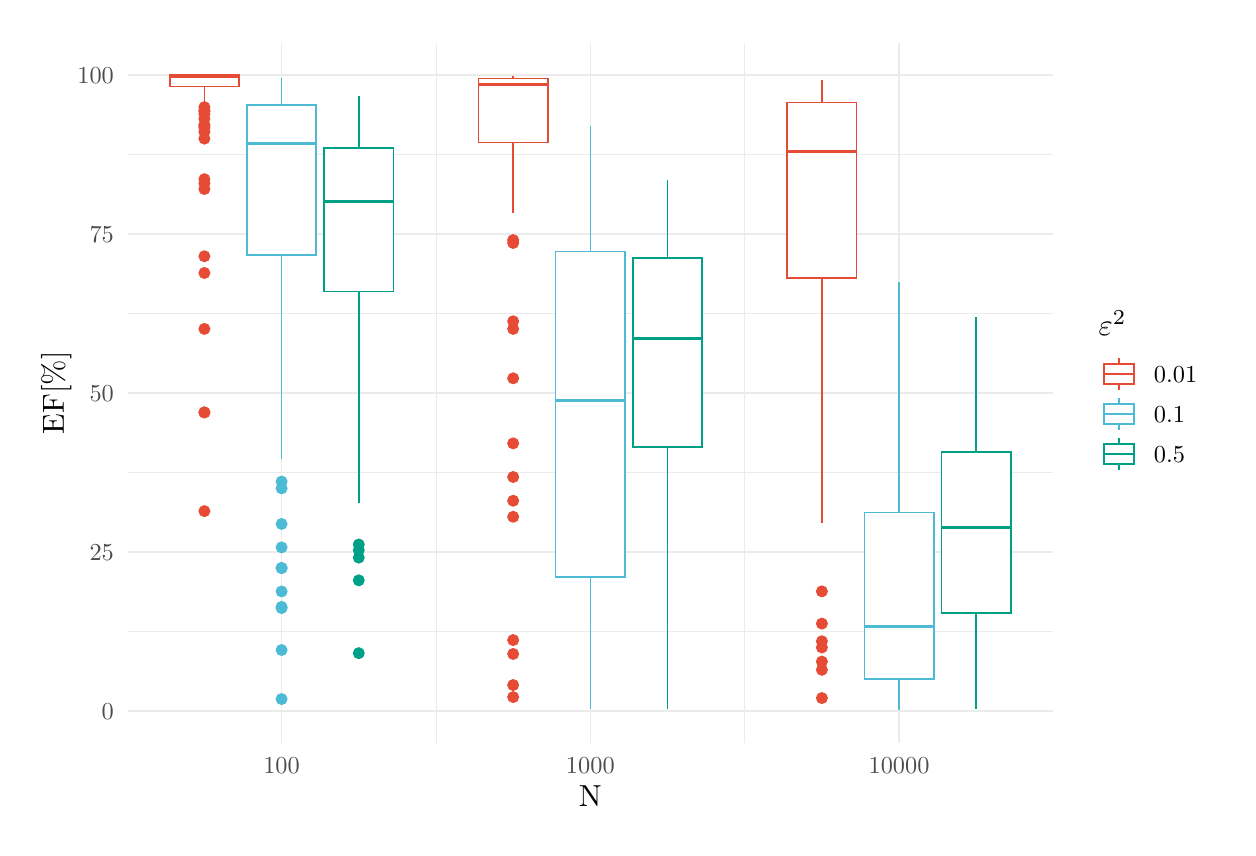
\begin{tikzpicture}[x=1pt,y=1pt]
\definecolor{fillColor}{RGB}{255,255,255}
\path[use as bounding box,fill=fillColor,fill opacity=0.00] (0,0) rectangle (433.62,289.08);
\begin{scope}
\path[clip] ( 36.11, 30.69) rectangle (370.53,283.58);
\definecolor{drawColor}{gray}{0.92}

\path[draw=drawColor,line width= 0.3pt,line join=round] ( 36.11, 70.92) --
	(370.53, 70.92);

\path[draw=drawColor,line width= 0.3pt,line join=round] ( 36.11,128.39) --
	(370.53,128.39);

\path[draw=drawColor,line width= 0.3pt,line join=round] ( 36.11,185.87) --
	(370.53,185.87);

\path[draw=drawColor,line width= 0.3pt,line join=round] ( 36.11,243.35) --
	(370.53,243.35);

\path[draw=drawColor,line width= 0.3pt,line join=round] (147.54, 30.69) --
	(147.54,283.58);

\path[draw=drawColor,line width= 0.3pt,line join=round] (259.10, 30.69) --
	(259.10,283.58);

\path[draw=drawColor,line width= 0.6pt,line join=round] ( 36.11, 42.18) --
	(370.53, 42.18);

\path[draw=drawColor,line width= 0.6pt,line join=round] ( 36.11, 99.66) --
	(370.53, 99.66);

\path[draw=drawColor,line width= 0.6pt,line join=round] ( 36.11,157.13) --
	(370.53,157.13);

\path[draw=drawColor,line width= 0.6pt,line join=round] ( 36.11,214.61) --
	(370.53,214.61);

\path[draw=drawColor,line width= 0.6pt,line join=round] ( 36.11,272.08) --
	(370.53,272.08);

\path[draw=drawColor,line width= 0.6pt,line join=round] ( 91.75, 30.69) --
	( 91.75,283.58);

\path[draw=drawColor,line width= 0.6pt,line join=round] (203.32, 30.69) --
	(203.32,283.58);

\path[draw=drawColor,line width= 0.6pt,line join=round] (314.88, 30.69) --
	(314.88,283.58);
\definecolor{drawColor}{RGB}{230,75,53}
\definecolor{fillColor}{RGB}{230,75,53}

\path[draw=drawColor,line width= 0.4pt,line join=round,line cap=round,fill=fillColor] ( 63.86,251.38) circle (  1.96);

\path[draw=drawColor,line width= 0.4pt,line join=round,line cap=round,fill=fillColor] ( 63.86,248.98) circle (  1.96);

\path[draw=drawColor,line width= 0.4pt,line join=round,line cap=round,fill=fillColor] ( 63.86,180.22) circle (  1.96);

\path[draw=drawColor,line width= 0.4pt,line join=round,line cap=round,fill=fillColor] ( 63.86,206.48) circle (  1.96);

\path[draw=drawColor,line width= 0.4pt,line join=round,line cap=round,fill=fillColor] ( 63.86,254.00) circle (  1.96);

\path[draw=drawColor,line width= 0.4pt,line join=round,line cap=round,fill=fillColor] ( 63.86,259.06) circle (  1.96);

\path[draw=drawColor,line width= 0.4pt,line join=round,line cap=round,fill=fillColor] ( 63.86,150.08) circle (  1.96);

\path[draw=drawColor,line width= 0.4pt,line join=round,line cap=round,fill=fillColor] ( 63.86,256.14) circle (  1.96);

\path[draw=drawColor,line width= 0.4pt,line join=round,line cap=round,fill=fillColor] ( 63.86,234.33) circle (  1.96);

\path[draw=drawColor,line width= 0.4pt,line join=round,line cap=round,fill=fillColor] ( 63.86,252.89) circle (  1.96);

\path[draw=drawColor,line width= 0.4pt,line join=round,line cap=round,fill=fillColor] ( 63.86,232.80) circle (  1.96);

\path[draw=drawColor,line width= 0.4pt,line join=round,line cap=round,fill=fillColor] ( 63.86,230.78) circle (  1.96);

\path[draw=drawColor,line width= 0.4pt,line join=round,line cap=round,fill=fillColor] ( 63.86,260.36) circle (  1.96);

\path[draw=drawColor,line width= 0.4pt,line join=round,line cap=round,fill=fillColor] ( 63.86,253.55) circle (  1.96);

\path[draw=drawColor,line width= 0.4pt,line join=round,line cap=round,fill=fillColor] ( 63.86,258.87) circle (  1.96);

\path[draw=drawColor,line width= 0.4pt,line join=round,line cap=round,fill=fillColor] ( 63.86,114.39) circle (  1.96);

\path[draw=drawColor,line width= 0.4pt,line join=round,line cap=round,fill=fillColor] ( 63.86,200.43) circle (  1.96);

\path[draw=drawColor,line width= 0.4pt,line join=round,line cap=round,fill=fillColor] ( 63.86,257.88) circle (  1.96);

\path[draw=drawColor,line width= 0.4pt,line join=round,line cap=round,fill=fillColor] ( 63.86,150.02) circle (  1.96);

\path[draw=drawColor,line width= 0.6pt,line join=round] ( 63.86,271.93) -- ( 63.86,272.07);

\path[draw=drawColor,line width= 0.6pt,line join=round] ( 63.86,267.84) -- ( 63.86,262.13);
\definecolor{fillColor}{RGB}{255,255,255}

\path[draw=drawColor,line width= 0.6pt,fill=fillColor] ( 51.31,271.93) --
	( 51.31,267.84) --
	( 76.41,267.84) --
	( 76.41,271.93) --
	( 51.31,271.93) --
	cycle;

\path[draw=drawColor,line width= 1.1pt] ( 51.31,271.62) -- ( 76.41,271.62);
\definecolor{drawColor}{RGB}{77,187,213}
\definecolor{fillColor}{RGB}{77,187,213}

\path[draw=drawColor,line width= 0.4pt,line join=round,line cap=round,fill=fillColor] ( 91.75,109.75) circle (  1.96);

\path[draw=drawColor,line width= 0.4pt,line join=round,line cap=round,fill=fillColor] ( 91.75, 79.34) circle (  1.96);

\path[draw=drawColor,line width= 0.4pt,line join=round,line cap=round,fill=fillColor] ( 91.75,101.28) circle (  1.96);

\path[draw=drawColor,line width= 0.4pt,line join=round,line cap=round,fill=fillColor] ( 91.75, 46.48) circle (  1.96);

\path[draw=drawColor,line width= 0.4pt,line join=round,line cap=round,fill=fillColor] ( 91.75, 64.19) circle (  1.96);

\path[draw=drawColor,line width= 0.4pt,line join=round,line cap=round,fill=fillColor] ( 91.75, 93.88) circle (  1.96);

\path[draw=drawColor,line width= 0.4pt,line join=round,line cap=round,fill=fillColor] ( 91.75, 93.76) circle (  1.96);

\path[draw=drawColor,line width= 0.4pt,line join=round,line cap=round,fill=fillColor] ( 91.75,122.61) circle (  1.96);

\path[draw=drawColor,line width= 0.4pt,line join=round,line cap=round,fill=fillColor] ( 91.75, 85.36) circle (  1.96);

\path[draw=drawColor,line width= 0.4pt,line join=round,line cap=round,fill=fillColor] ( 91.75, 79.78) circle (  1.96);

\path[draw=drawColor,line width= 0.4pt,line join=round,line cap=round,fill=fillColor] ( 91.75,125.06) circle (  1.96);

\path[draw=drawColor,line width= 0.6pt,line join=round] ( 91.75,261.10) -- ( 91.75,270.84);

\path[draw=drawColor,line width= 0.6pt,line join=round] ( 91.75,206.87) -- ( 91.75,133.20);
\definecolor{fillColor}{RGB}{255,255,255}

\path[draw=drawColor,line width= 0.6pt,fill=fillColor] ( 79.20,261.10) --
	( 79.20,206.87) --
	(104.30,206.87) --
	(104.30,261.10) --
	( 79.20,261.10) --
	cycle;

\path[draw=drawColor,line width= 1.1pt] ( 79.20,247.32) -- (104.30,247.32);
\definecolor{drawColor}{RGB}{0,160,135}
\definecolor{fillColor}{RGB}{0,160,135}

\path[draw=drawColor,line width= 0.4pt,line join=round,line cap=round,fill=fillColor] (119.64,102.33) circle (  1.96);

\path[draw=drawColor,line width= 0.4pt,line join=round,line cap=round,fill=fillColor] (119.64,100.27) circle (  1.96);

\path[draw=drawColor,line width= 0.4pt,line join=round,line cap=round,fill=fillColor] (119.64, 97.58) circle (  1.96);

\path[draw=drawColor,line width= 0.4pt,line join=round,line cap=round,fill=fillColor] (119.64, 89.37) circle (  1.96);

\path[draw=drawColor,line width= 0.4pt,line join=round,line cap=round,fill=fillColor] (119.64, 63.06) circle (  1.96);

\path[draw=drawColor,line width= 0.6pt,line join=round] (119.64,245.64) -- (119.64,264.45);

\path[draw=drawColor,line width= 0.6pt,line join=round] (119.64,193.75) -- (119.64,117.25);
\definecolor{fillColor}{RGB}{255,255,255}

\path[draw=drawColor,line width= 0.6pt,fill=fillColor] (107.09,245.64) --
	(107.09,193.75) --
	(132.20,193.75) --
	(132.20,245.64) --
	(107.09,245.64) --
	cycle;

\path[draw=drawColor,line width= 1.1pt] (107.09,226.34) -- (132.20,226.34);
\definecolor{drawColor}{RGB}{230,75,53}
\definecolor{fillColor}{RGB}{230,75,53}

\path[draw=drawColor,line width= 0.4pt,line join=round,line cap=round,fill=fillColor] (175.43,126.72) circle (  1.96);

\path[draw=drawColor,line width= 0.4pt,line join=round,line cap=round,fill=fillColor] (175.43, 62.77) circle (  1.96);

\path[draw=drawColor,line width= 0.4pt,line join=round,line cap=round,fill=fillColor] (175.43,211.28) circle (  1.96);

\path[draw=drawColor,line width= 0.4pt,line join=round,line cap=round,fill=fillColor] (175.43, 47.19) circle (  1.96);

\path[draw=drawColor,line width= 0.4pt,line join=round,line cap=round,fill=fillColor] (175.43,182.99) circle (  1.96);

\path[draw=drawColor,line width= 0.4pt,line join=round,line cap=round,fill=fillColor] (175.43,212.32) circle (  1.96);

\path[draw=drawColor,line width= 0.4pt,line join=round,line cap=round,fill=fillColor] (175.43, 51.54) circle (  1.96);

\path[draw=drawColor,line width= 0.4pt,line join=round,line cap=round,fill=fillColor] (175.43,138.87) circle (  1.96);

\path[draw=drawColor,line width= 0.4pt,line join=round,line cap=round,fill=fillColor] (175.43,180.21) circle (  1.96);

\path[draw=drawColor,line width= 0.4pt,line join=round,line cap=round,fill=fillColor] (175.43, 67.79) circle (  1.96);

\path[draw=drawColor,line width= 0.4pt,line join=round,line cap=round,fill=fillColor] (175.43,162.38) circle (  1.96);

\path[draw=drawColor,line width= 0.4pt,line join=round,line cap=round,fill=fillColor] (175.43,112.33) circle (  1.96);

\path[draw=drawColor,line width= 0.4pt,line join=round,line cap=round,fill=fillColor] (175.43,118.13) circle (  1.96);

\path[draw=drawColor,line width= 0.6pt,line join=round] (175.43,270.66) -- (175.43,271.72);

\path[draw=drawColor,line width= 0.6pt,line join=round] (175.43,247.63) -- (175.43,222.28);
\definecolor{fillColor}{RGB}{255,255,255}

\path[draw=drawColor,line width= 0.6pt,fill=fillColor] (162.88,270.66) --
	(162.88,247.63) --
	(187.98,247.63) --
	(187.98,270.66) --
	(162.88,270.66) --
	cycle;

\path[draw=drawColor,line width= 1.1pt] (162.88,268.45) -- (187.98,268.45);
\definecolor{drawColor}{RGB}{77,187,213}

\path[draw=drawColor,line width= 0.6pt,line join=round] (203.32,208.19) -- (203.32,253.54);

\path[draw=drawColor,line width= 0.6pt,line join=round] (203.32, 90.60) -- (203.32, 43.02);

\path[draw=drawColor,line width= 0.6pt,fill=fillColor] (190.77,208.19) --
	(190.77, 90.60) --
	(215.87, 90.60) --
	(215.87,208.19) --
	(190.77,208.19) --
	cycle;

\path[draw=drawColor,line width= 1.1pt] (190.77,154.31) -- (215.87,154.31);
\definecolor{drawColor}{RGB}{0,160,135}

\path[draw=drawColor,line width= 0.6pt,line join=round] (231.21,205.74) -- (231.21,233.88);

\path[draw=drawColor,line width= 0.6pt,line join=round] (231.21,137.67) -- (231.21, 42.94);

\path[draw=drawColor,line width= 0.6pt,fill=fillColor] (218.66,205.74) --
	(218.66,137.67) --
	(243.76,137.67) --
	(243.76,205.74) --
	(218.66,205.74) --
	cycle;

\path[draw=drawColor,line width= 1.1pt] (218.66,176.71) -- (243.76,176.71);
\definecolor{drawColor}{RGB}{230,75,53}
\definecolor{fillColor}{RGB}{230,75,53}

\path[draw=drawColor,line width= 0.4pt,line join=round,line cap=round,fill=fillColor] (286.99, 57.04) circle (  1.96);

\path[draw=drawColor,line width= 0.4pt,line join=round,line cap=round,fill=fillColor] (286.99, 65.12) circle (  1.96);

\path[draw=drawColor,line width= 0.4pt,line join=round,line cap=round,fill=fillColor] (286.99, 60.01) circle (  1.96);

\path[draw=drawColor,line width= 0.4pt,line join=round,line cap=round,fill=fillColor] (286.99, 85.39) circle (  1.96);

\path[draw=drawColor,line width= 0.4pt,line join=round,line cap=round,fill=fillColor] (286.99, 73.74) circle (  1.96);

\path[draw=drawColor,line width= 0.4pt,line join=round,line cap=round,fill=fillColor] (286.99, 46.83) circle (  1.96);

\path[draw=drawColor,line width= 0.4pt,line join=round,line cap=round,fill=fillColor] (286.99, 67.36) circle (  1.96);

\path[draw=drawColor,line width= 0.6pt,line join=round] (286.99,262.03) -- (286.99,270.08);

\path[draw=drawColor,line width= 0.6pt,line join=round] (286.99,198.53) -- (286.99,110.21);
\definecolor{fillColor}{RGB}{255,255,255}

\path[draw=drawColor,line width= 0.6pt,fill=fillColor] (274.44,262.03) --
	(274.44,198.53) --
	(299.54,198.53) --
	(299.54,262.03) --
	(274.44,262.03) --
	cycle;

\path[draw=drawColor,line width= 1.1pt] (274.44,244.33) -- (299.54,244.33);
\definecolor{drawColor}{RGB}{77,187,213}

\path[draw=drawColor,line width= 0.6pt,line join=round] (314.88,113.84) -- (314.88,197.09);

\path[draw=drawColor,line width= 0.6pt,line join=round] (314.88, 53.80) -- (314.88, 42.37);

\path[draw=drawColor,line width= 0.6pt,fill=fillColor] (302.33,113.84) --
	(302.33, 53.80) --
	(327.43, 53.80) --
	(327.43,113.84) --
	(302.33,113.84) --
	cycle;

\path[draw=drawColor,line width= 1.1pt] (302.33, 72.66) -- (327.43, 72.66);
\definecolor{drawColor}{RGB}{0,160,135}

\path[draw=drawColor,line width= 0.6pt,line join=round] (342.77,135.84) -- (342.77,184.37);

\path[draw=drawColor,line width= 0.6pt,line join=round] (342.77, 77.54) -- (342.77, 42.91);

\path[draw=drawColor,line width= 0.6pt,fill=fillColor] (330.22,135.84) --
	(330.22, 77.54) --
	(355.32, 77.54) --
	(355.32,135.84) --
	(330.22,135.84) --
	cycle;

\path[draw=drawColor,line width= 1.1pt] (330.22,108.44) -- (355.32,108.44);
\end{scope}
\begin{scope}
\path[clip] (  0.00,  0.00) rectangle (433.62,289.08);
\definecolor{drawColor}{gray}{0.30}

\node[text=drawColor,anchor=base east,inner sep=0pt, outer sep=0pt, scale=  0.88] at ( 31.16, 39.15) {0};

\node[text=drawColor,anchor=base east,inner sep=0pt, outer sep=0pt, scale=  0.88] at ( 31.16, 96.63) {25};

\node[text=drawColor,anchor=base east,inner sep=0pt, outer sep=0pt, scale=  0.88] at ( 31.16,154.10) {50};

\node[text=drawColor,anchor=base east,inner sep=0pt, outer sep=0pt, scale=  0.88] at ( 31.16,211.58) {75};

\node[text=drawColor,anchor=base east,inner sep=0pt, outer sep=0pt, scale=  0.88] at ( 31.16,269.05) {100};
\end{scope}
\begin{scope}
\path[clip] (  0.00,  0.00) rectangle (433.62,289.08);
\definecolor{drawColor}{gray}{0.30}

\node[text=drawColor,anchor=base,inner sep=0pt, outer sep=0pt, scale=  0.88] at ( 91.75, 19.68) {100};

\node[text=drawColor,anchor=base,inner sep=0pt, outer sep=0pt, scale=  0.88] at (203.32, 19.68) {1000};

\node[text=drawColor,anchor=base,inner sep=0pt, outer sep=0pt, scale=  0.88] at (314.88, 19.68) {10000};
\end{scope}
\begin{scope}
\path[clip] (  0.00,  0.00) rectangle (433.62,289.08);
\definecolor{drawColor}{RGB}{0,0,0}

\node[text=drawColor,anchor=base,inner sep=0pt, outer sep=0pt, scale=  1.10] at (203.32,  7.64) {N};
\end{scope}
\begin{scope}
\path[clip] (  0.00,  0.00) rectangle (433.62,289.08);
\definecolor{drawColor}{RGB}{0,0,0}

\node[text=drawColor,rotate= 90.00,anchor=base,inner sep=0pt, outer sep=0pt, scale=  1.10] at ( 13.08,157.13) {EF[\%]};
\end{scope}
\begin{scope}
\path[clip] (  0.00,  0.00) rectangle (433.62,289.08);
\definecolor{drawColor}{RGB}{0,0,0}

\node[text=drawColor,anchor=base west,inner sep=0pt, outer sep=0pt, scale=  1.10] at (387.03,177.78) {$\varepsilon^2$};
\end{scope}
\begin{scope}
\path[clip] (  0.00,  0.00) rectangle (433.62,289.08);
\definecolor{drawColor}{RGB}{230,75,53}

\path[draw=drawColor,line width= 0.6pt] (394.25,158.20) --
	(394.25,160.37);

\path[draw=drawColor,line width= 0.6pt] (394.25,167.59) --
	(394.25,169.76);
\definecolor{fillColor}{RGB}{255,255,255}

\path[draw=drawColor,line width= 0.6pt,fill=fillColor] (388.83,160.37) rectangle (399.67,167.59);

\path[draw=drawColor,line width= 0.6pt] (388.83,163.98) --
	(399.67,163.98);
\end{scope}
\begin{scope}
\path[clip] (  0.00,  0.00) rectangle (433.62,289.08);
\definecolor{drawColor}{RGB}{77,187,213}

\path[draw=drawColor,line width= 0.6pt] (394.25,143.74) --
	(394.25,145.91);

\path[draw=drawColor,line width= 0.6pt] (394.25,153.14) --
	(394.25,155.31);
\definecolor{fillColor}{RGB}{255,255,255}

\path[draw=drawColor,line width= 0.6pt,fill=fillColor] (388.83,145.91) rectangle (399.67,153.14);

\path[draw=drawColor,line width= 0.6pt] (388.83,149.53) --
	(399.67,149.53);
\end{scope}
\begin{scope}
\path[clip] (  0.00,  0.00) rectangle (433.62,289.08);
\definecolor{drawColor}{RGB}{0,160,135}

\path[draw=drawColor,line width= 0.6pt] (394.25,129.29) --
	(394.25,131.46);

\path[draw=drawColor,line width= 0.6pt] (394.25,138.69) --
	(394.25,140.85);
\definecolor{fillColor}{RGB}{255,255,255}

\path[draw=drawColor,line width= 0.6pt,fill=fillColor] (388.83,131.46) rectangle (399.67,138.69);

\path[draw=drawColor,line width= 0.6pt] (388.83,135.07) --
	(399.67,135.07);
\end{scope}
\begin{scope}
\path[clip] (  0.00,  0.00) rectangle (433.62,289.08);
\definecolor{drawColor}{RGB}{0,0,0}

\node[text=drawColor,anchor=base west,inner sep=0pt, outer sep=0pt, scale=  0.88] at (406.98,160.95) {0.01};
\end{scope}
\begin{scope}
\path[clip] (  0.00,  0.00) rectangle (433.62,289.08);
\definecolor{drawColor}{RGB}{0,0,0}

\node[text=drawColor,anchor=base west,inner sep=0pt, outer sep=0pt, scale=  0.88] at (406.98,146.50) {0.1};
\end{scope}
\begin{scope}
\path[clip] (  0.00,  0.00) rectangle (433.62,289.08);
\definecolor{drawColor}{RGB}{0,0,0}

\node[text=drawColor,anchor=base west,inner sep=0pt, outer sep=0pt, scale=  0.88] at (406.98,132.04) {0.5};
\end{scope}
\end{tikzpicture}
%
        }
        \caption{Empirical \acrshort{ef} for the setup of \Cref{ex:ess_failure} for varying sample sizes $N$ and $\varepsilon^{2}$. In all scenarios the second moment $\rho$ is infinite, thus high \acrshortpl{ef} are misleading us to believe that importance sampling performs well when it does not.}
        \label{fig:ess_failure}
    \end{figure}


\end{example}

As an alternative, we may want to assess whether importance sampling has converged through the empirical variance of $\hat \zeta$, i.e., 
$$
\widehat\var \left( \hat\zeta \right) = \frac{1}{N}\left(\frac{1}{N} \sum_{i = 1}^N w_{i}^{2} f(X^{i})^{2} - \hat \zeta^{2}\right)
$$
is, while seemingly natural, flawed \citep{Chatterjee2018Sample}.
Indeed, the authors show that for any given threshold $\epsilon$ we may find an $N$ which only depends on $\epsilon$, such that the probability that the empirical variance exceeds $\epsilon$ for this $N$ is small. This is summarized in the following theorem.

\begin{theorem}[{\cite[Theorem 2.1]{Chatterjee2018Sample}}]
    Given any $\epsilon > 0$, there exists $N \leq \epsilon^{-2} 2^{1 + \epsilon^{-3}}$ such that the following is true. Take any $\G$ and $\P$ as in \Cref{thm:chatterje2018Thm1}, and any $f: \mathcal X \to \R$ such that $ \lVert f \rVert_{L^{2}(\P)} \leq 1.$ Then 
    $$
        \mathbb P \left( \widehat \var \left( \hat \zeta \right) < \epsilon\right) \geq 1 - 4 \epsilon.
    $$
    \todo{make $\zeta$ depend on $N$?}
\end{theorem}

The problem here is that $N$ does not depend on $\G$ and $\P$, so we may choose $\G$ almost singular to $\P$. \todo{continue}

Thus using the empirical variance as a threshold for convergence should be avoided. As a remedy \citep{Chatterjee2018Sample} suggest the heuristic $q_{N} = \E Q_{N}$ where
$$
Q_{N} = \max_{1\leq i\leq N} W_{i}.
$$
\todoTH{more details}
This judges whether importance sampling has collapsed to just a few particles and is itself amenable to Monte-Carlo integration, though this requires multiple runs of importance sampling and so may be prohibitively expensive in practice.

In the following sections, we will predominantly take the position that we are interested in finding a good particle approximation $\hat\P_{N}$ of the form \Cref{eq:is-particle-approximation} over finding the optimal proposal $\G^{\ast}$ \Cref{prop:minimum_MSE_IS} and assume that the importance sampling weights can only be evaluated up to a constant. 
\todo{more clearly distinguish arguments for the two assumptions}
This has several reasons: First of all, for most problems considered in this thesis $\P$ is usually a conditional distribution, e.g. $\P = \mathbb P^{X|Y=y}$ for states $X$ and observations $Y$ in the \acrshort{ssm} context. Should the appropriate densities exist, evaluating the weights amounts to calculating 
$$
\rnd{\mathbb P^{X| Y= y}}{\G}(x) = \frac{p(x|y)}{g(x)} = \frac{p(y|x)p(x)}{g(x)p(y)} \propto \frac{p(y|x)p(x)}{g(x)}.
$$
In these situations $p(y) = \int p(x,y)\d x$ is usually intractable. For $\G^{\ast}$ we are in the same situation, where the evaluation of the integration constant $\P \lvert f \rvert$ is infeasible, but the density $\lvert f(x)\rvert p(x)$ is available.
% do not focus on a single f
Second, focusing on the particle approximation allows us to consider multiple test functions $f$, e.g. focus on different marginals of $\P$, which is usually what practitioners are interested in. 
% simplify notation: P always target, G always proposal
Finally, this allows us to simplify the notation used in this thesis. $\P$ will always be the probability measure of interest and $\G$ the proposal. In later parts of this thesis, we will predominantly perform Gaussian importance sampling, i.e. $\G = \mathcal N(\mu, \Sigma)$, hence a handy mnemonic is to think of $\G$ as a \textbf{G}aussian proposal.

\subsection{\texorpdfstring{\Acrfull{la}}{Laplace approximation}}
\label{subsec:la}

The \acrfull{la} goes back to Laplace \citep{Laplace1986Memoir} who invented the technique to approximate moments of otherwise intractable distributions. Since \citep{Tierney1986Accurate,Tierney1989Fully} rediscovered its use to approximate posterior means and variances, it has been a staple method for approximate inference.
The method is based on a second-order Taylor series expansion of the log target density $\log p(x)$ around its mode $\hat x$, i.e. matching mode and curvature. Assuming the density is sufficiently smooth, we have
\begin{align}
    \label{eq:LA_approximation}
\log p(x) \approx \log p(\hat x) + \underbrace{\nabla_{x} \log p (\hat x)}_{= 0} \left( x - \hat x \right) + \frac{1}{2} (x - \hat x)^{T} H (x - \hat x)
\end{align}
where $H$ is the Hessian of $\log p$ evaluated at $\hat x$. As $\log p (\hat x)$ does not depend on $x$, the right-hand side can be seen (up to additive constants) as the density of a Gaussian distribution with mean $\hat x$ and covariance matrix $\Sigma = - H^{-1}$. Thus using $\G = \mathcal N (\hat x, -H^{-1})$ as a proposal in importance sampling seems promising. 
% degenerate case when $H$ is not PSD
If $\hat x$ is the unique global mode of $p$ and $H$ is negative definite, the \gls{la} yields an actual Gaussian distribution. 
\todo{else?}
% numerics
To obtain the \acrshort{la} in practice, a Newton-Raphson scheme may be used, which conveniently tracks $H$ as well. 

% advantages / disadvantages
The main advantage of the \gls{la} is that it is usually fast to obtain and, for sufficiently well-behaved distributions on a moderate dimensional space, provides reasonably high \gls{ess}. Additionally, the Newton-Raphson iterations to find the mode and Hessian are robust and require no simulation, unlike the other methods discussed further below.
For the \glspl{ssm} we consider in this thesis, the numerical methods can be implemented using the Kalman filter and smoother \citep{Shephard1997Likelihood,Durbin1997Monte}, even in the degenerate case where $H$ is indefinite \citep{Jungbacker2007Monte}, see also \Cref{subsec:glssm-approach}.
\todo{more theoretical background on LA?}

However, as the \gls{la} is a local approximation, it may be an inappropriate description of the global behavior of the target, see \Cref{ex:la_failure} for a breakdown of \gls{la} and the simulation studies presented in \Cref{sec:simulation_studies}. 
Additionally, even if \gls{la} works in principle, its \gls{ess} will usually degenerate quickly once the dimension increases whereas the \gls{cem} and \gls{eis} do so at a slower pace.

\glsreset{cem}
\subsection{The \texorpdfstring{\Acrfull{cem}}{Cross-Entropy method}}
\label{subsec:cem}
Recall from our discussion surrounding \Cref{thm:chatterje2018Thm1} that for importance sampling to be effective, we should have a small \acrshort{kld} between the target $\P$ and the proposal $\G$. As the \acrshort{kld} depends on global properties, i.e. the Radon-Nikodym derivative $\rnd{\P}{\G}$, minimizing it should lead to a global approximation of $\P$.
The \gls{cem}\citep{Rubinstein1999CrossEntropy,Rubinstein2004CrossEntropy} implements this idea and selects from a parametric family $ \left( \G_{\psi} \right)_{\psi \in \Psi}$ of proposals the one that minimizes the \gls{kld} to the target. Thus, the \acrshort{cem} finds $\psi_{\text{CE}}$ which solves the following optimization problem

\begin{align*}
    \psi_{\text{CE}} &= \argmin_{\psi \in \Psi} \Dkl{\P}{\G_{\psi}} \\
    &= \argmin_{\psi \in \Psi} \int \log \frac{\d \P}{\d\G_{\psi}} \d \P.
\end{align*}
As the \acrshort{kld} is convex in both arguments, 
If $\P$ and $\G_{\psi}$ possess densities $p$ and $g_{\psi}$ w.r.t. some common measure $\mu$, the same for all $\psi$, we may reformulate the optimization problem to maximize the cross-entropy between $p$ and $g_{\psi}$ instead:
\begin{align}
    \begin{split}
    \psi_{\text{CE}} &= \argmin_{\psi \in \Psi} \int  p(x)\log p(x) \d \mu(x) - \int p(x)\log g_{\psi} \d \mu(x) \\ 
    &= \argmax_{\psi \in \Psi} \int p(x) \log g_{\psi}(x) \d \mu(x)
    \end{split} \label{eq:ce_argmax}.
\end{align}
\todoTH{discuss existence, borderline cases}
Note that the first integral does not depend on $\psi$. The assumption of such a dominating measure is not restrictive: otherwise the \gls{kld} is infinite. 

%
%As $\P$ is usually intractable, so is $\psi_{\text{CE}}$. However, the integral \Cref{eq:ce_argmax} is amenable to importance sampling: Given a proposal $\G$, we may estimate it by
%\begin{align}
%\hat\psi_{\text{CE}} &= \argmax_{\psi \in \Psi} \hat \P_{N} \log g_{\psi} = \argmax_{\psi\in\Psi} \sum_{i = 1}^{N}W^{i}\log g_{\psi}(X^{i}) \label{eq:ce-M-estimator}
%\end{align}
%where $X_1, \dots, X_N \iid \G$. 
%Thus $\hat \psi_{\text{CE}}$ is an M-estimator and we may analyze its asymptotic behavior by standard methods, see e.g. \citep[Chapter 5]{VanderVaart2000Asymptotic}.
%
%\todo{rework this: consistency for non-EF proposals (there use VdV and potentially technical assumptions, then special case of EF with Brown)}
%% M-estimator behaviour 
%
%\begin{theorem}[consistencty of $\hat\psi_{\text{CE}}$]
%    \label{thm:ce-m-estimator}
%    Assume the following technical conditions apply:
%    \begin{itemize}
%        \item[A1] Uniform consistency of importance sampling
%            $$\sup_{\psi \in \Psi}\lVert \hat \G_N (w\log g_\psi) - \G(w \log g_\psi) \rVert \stackrel{P}{\to} 0$$ 
%        \item[A2] Regularity condition
%            $$ \partial_\psi \P \left(\log g_\theta\right) = \P \left(\partial_\theta \log g_\theta\right) $$
%            for all $\psi \in \Psi$
%        \item[A3] positive definite misspecified Fisher information
%            $$ \P \left(\left(\partial_\psi \log g_\theta\right)\left(\partial_\theta \log g_\theta\right)^T\right) > 0$$
%    \end{itemize}
%
%    Then $\hat\psi_{\text{CE}}$ is a consistent estimator of $\psi_{\text{CE}}$.
%\end{theorem}
%
%\begin{theorem}[asymptotic normality of $\hat\psi_{\text{CE}}$]
%    
%\end{theorem}

% analytical solution, MLE
\todo{make theorem, proof}
An attractive property of the \gls{cem} is that if $\G_{\psi}$ form an exponential family with natural parameter $\psi \in \R^{p}$, the optimal $\psi_{\text{CE}}$ only depends on the expected value $\P [T]$. Indeed, for $\log g_{\psi}(x) = \log h(x) - \log Z(\psi) + \psi^{T} T(x)$ we have 
$$
\int p(x) \log g_{\psi}(x) \d \mu(x) = \P \log h - \log Z(\psi) + \psi^{T} \P T.
$$
As $\log Z(\psi)$ is the cumulant-generating function of $\G_{\psi}$ it is smooth. Thus the optimal $\psi_{\text{CE}}$ solves
$$
\P T = \nabla_{\psi} \log Z(\pce) = \G_{\pce}T,
$$
and the task at hand reduces to matching the moments of the sufficient statistic of the target and proposal.
In many cases, this system of equations can be solved analytically or by gradient descent algorithms.

While $\P T$ is usually not available, it is itself amenable to importance sampling. Given a proposal $\G$ we may estimate $\P T$ by $\hat\P_N T = \sum_{i = 1}^{N} W^{i} T(X^{i})$ for $X^{1}, \dots, X^{N} \iid \G$ and auto-normalized importance sampling weights $W^{i}$ and in turn estimate $\psi_{\text{CE}}$ by $\hat \psi_{\text{CE}}$ solving
$$
\hat \P_N T = \G_{\hpce} T.
$$
% proof: appeal to vdV, pd ensures that M(\theta) is convex, so global maximum unique and well separated
Thus $\hat\psi_{\text{CE}}$ is a Z-estimator, i.e. an estimator that arises from solving a random system of equations, and we can analyze its asymptotic behavior using standard results from the theory of Z-estimators. 
The following theorem of \citep{VanderVaart2000Asymptotic} will be useful in analyzing the asymptotic behavior of the estimators we consider in this thesis. We state it here, using our notation, for completeness.

\begin{theorem}[asymptotic variance of Z-estimators, {\citep[Theorem 5.21]{VanderVaart2000Asymptotic}}]
    \label{thm:clt_z_est_vdv}
    For every $\psi$ in an open subset of $\R^{k}$, let $x \mapsto f_{\psi}(x)$ be a measurable vector-valued function such that, for every $\psi_{1}$ and $\psi_{2}$ in a neighborhood of $\psi_{0}$ and a measurable function $\dot f$ with $\G \dot f < \infty$,
    \begin{align}
    \label{eq:clt-vdv-local-lipschitz}
    \lVert f_{\psi_{1}}(x) - f_{\psi_{2}}(x)\rVert \leq \dot f(x) \lVert \psi_{1} - \psi_{2}\rVert \tag{LL}.
    \end{align}

    Assume that $\G \lVert f_{\psi_{0}}\rVert < \infty$ and that the map $\psi \mapsto \G f_{\psi}$ is differentiable at $\psi_{0}$, with nonsingular derivative matrix $B^{-1}$. Let $X_{1}, \dots, X_{N} \iid \G$ and $\hat \G_{N} = \sum_{i = 1}^{N} \delta_{X^{i}}$. If $\hat\psi_{N}$ fulfills $\hat\G_{N} f_{\hat\psi_{N}} = o_{P} \left( N^{-\frac{1}{2}} \right)$, and $\hat\psi_{N} \to \psi_{0}$ in probability, then
    \begin{align}
        \label{eq:clt-vdv}
        \sqrt{N} \left( \hat\psi_{N} - \psi_{0} \right) \Dto \mathcal N(0, BMB^{T}),
    \end{align}
    where $M = \G f_{\psi_{0}} f_{\psi_{0}^{T}}$.
\end{theorem}

\begin{notation}[central limit theorem for Z-estimators]
    \label{not:notation-clt}
    The central limit theorems derived in this and the next section will make frequent use of \Cref{thm:clt_z_est_vdv}. We will use the following consistent notation in the statement of theorems and their proofs:
    \begin{itemize}
        \item $f_\psi(x): \R^{k} \to \R^{k}$ the estimating equation              
        \item $B = \left(\G\partial_{\psi} f_{\psi}\right)^{-1}$ the bread matrix
        \item $M = \G f_{\psi}f_{\psi}^{T}$ the meat matrix
        \item $V = BMB$ the asymptotic covariance matrix
        \item $\log g_{\psi}(x) = \psi^{T}T(x) + \log h(x) - \log Z(\psi)$ the density of the natural exponential family considered
        \item $\dot z (\psi) = \nabla_{\psi}\log Z(\psi) = \G_{\psi} T$ the derivative of the log-normalizing constant $\psi \mapsto \log Z(\psi)$
        \item $\ddot z(\psi) = \partial_{\psi} \dot z(\psi) =\cov_{\G_{\psi}}T$ the Hessian of the log-normalizing constant $\psi \mapsto \log Z(\psi)$
    \end{itemize}
    The naming of $B$ and $M$ stems from the sandwich estimator \citep{White1982Maximum}, where the bread $B$ is the Jacobian of the estimating equations $\P f_{\psi} = 0$ and the meat $M$ is the covariance matrix of $f_{\psi}$ under $\P$, thus making a \glqq{}meat sandwich\grqq{}.
\end{notation}

\todo{discussion on relevance and novelty of these results}
\begin{theorem}[consistency of $\hat \psi_{\text{CE}}$]
    \label{thm:ce-consistent}
    \todo{from van der Vaart/Casella Berger}
\end{theorem}


\begin{theorem}[asymptotic normality of $\hat \psi_{\text{CE}}$]
    \label{thm:ce-clt}
    %\todo{require unique solution?}
    Let $\G_{\psi}$ form a natural exponential family with densities $g_{\psi}(x) = \frac{h(x)}{Z(\psi)} \exp \left( \psi^{T}T(x)\right) $ w.r.t. $\mu$. Let $\G, \P$ be two other probability measures such that $\G \ll \P$ and let $W = \frac{\d \P}{\d \G}$ be the normalized importance sampling weights. 
    Suppose further that 
    \begin{enumerate}[label={\bfseries(A{\arabic*})}]
        \item\label{it:exist-unique-psice} $\G_{\hpce} T = \hat\P_{N} T$ $\mu$-a.s. has a unique solution $\hpce$,
        \item\label{it:zdot-ll} $\psi \mapsto \nabla_\psi \log Z(\psi)$ is locally Lipschitz around $\psi_{\text{CE}}$,
        \item\label{it:w-t-wt-L2} $W,T$ and $WT$ possess finite second moments  w.r.t. $\G$,
        \item\label{it:FI-psd} the Fisher information $I(\psi_{\text{CE}})$ is positive definite and equal to $-\ddot z(\pce)$, additionally $\psi \mapsto I(\psi)$ is continuous, and
        \item\label{it:ce-regularity} the regularity conditions of \Cref{thm:ce-consistent} hold.
    \end{enumerate}

    Then, as $N$ goes to $\infty$,
    $$
        \sqrt{N} \left(\hat\psi_\text{CE} - \psi_{\text{CE}}\right) \Dto \mathcal N \left(0, V_{\text{CE}}\right)
    $$
    where 
    $$
    V_{\text{CE}} = B_\ce M_\ce B_\ce,%I(\psi_{\text{CE}})^{-1}  \text{Cov}_{\G} \left( W (T - \G_{\pce}T) \right) I(\psi_{\text{CE}})^{-1},
    $$
    with 
    \begin{align*}
        B_{\ce} &= I(\pce)^{-1}, \\
        M_{\ce} &= \cov_{\G} \left( W (T - \G_{\pce}T) \right).
    \end{align*}
    Moreover $\G (W(T - \G_{\pce}T))) = 0$, so we may estimate $V_{\text{CE}}$ consistently by plug-in:
    $$
    \hat V_{\text{CE}} = I(\hat\psi_{\text{CE}})^{-1}  \left(\sum_{i = 1}^N W^{2}_{i} \left(T(X^{i}) - \G_{\hpce}T \right)\left(T(X^{i}) - \G_{\hpce} T\right)^{T} \right)I(\hat\psi_{\text{CE}})^{-1}.
    $$
\end{theorem}

\begin{proof} We check that the conditions of the central limit theorem for Z-estimators (\Cref{thm:clt_z_est_vdv}) are fulfilled. This proof uses the notation established in \Cref{not:notation-clt}. Consider the estimating equations for $\pce$ 
    $$x\mapsto f_\psi(x) = \nabla_{\psi} \left(w(x)\log g_{\psi}(x)\right) = w(x) T(x) - w(x) \dot z (\psi),$$ where $w(x)$ are the unnormalized importance sampling weights. 
    By \ref{it:exist-unique-psice} $\hat \P_{N} f_{\hpce} = 0$ $\mu$-a.s., so it remains to show that $\hpce \to \pce$  in probability, which is implied by \Cref{thm:ce-consistent}.
    
    As $$\left\lVert f_{\psi_1}(x) - f_{\psi_2}(x)\right\rVert = w(x) \left\lVert \dot z (\psi_1) - \dot z(\psi_2)\right\rVert$$ for all $\psi_{1}, \psi_{2}\in \Psi$,  $\G w < \infty $ and \ref{it:zdot-ll} imply the local Lipschitz condition \Cref{eq:clt-vdv-local-lipschitz} in \Cref{thm:clt_z_est_vdv}.
    Furthermore, by \ref{it:w-t-wt-L2} it holds
    %\todo{fix: no triangle equation (squared norm)}
    $$
    \G \left\lVert f_\psi \right\rVert^2 \leq \G w^2 \left\lVert \dot z(\psi) \right\rVert ^2  + 2 \lVert \dot z(\psi) \rVert \G \lVert wT\rVert + \G \left\lVert wT\right\rVert^2 < \infty.
    $$

    Additionally $\psi \mapsto\G f_\psi = (\G w) \dot z (\psi) + \G wT$ is differentiable everywhere, with Jacobian $(\G w) \ddot z(\psi)$, where  $\ddot z(\psi) = \partial_\psi \dot z(\psi)$ is the Hessian of the cumulant generating function, which equals the negative Fisher information $-I(\pce)$ as $\G_{\psi}, \psi \in \Psi$ form a natural exponential family and the regularity conditions \ref{it:ce-regularity} allow differentiation under the integral.
    Thus we see that 
    $$
    \G f_{\pce} = \P \left( \dot z(\pce) + T \right) = \dot z (\pce) + \P T = 0,
    $$
    by definition of $\pce$, so $$\text{Cov}_{\G} \left( w(T - \nabla_{\pce} \log Z (\pce)) \right) = \text{Cov}_{\G}(f_{\pce}) = \G f_{\pce}f_{\pce}^{T}.$$
    As $W = \frac{w}{\G w}$
    By \Cref{eq:clt-vdv} the asymptotic covariance matrix is 
    $$
    V_{\ce} = B_{\ce}M_{\ce}B_{\ce}
    $$
    which shows the asymptotic normality. 

    Estimating $B_{\ce}$ by $\hat B_{\ce}= I(\hpce)$ and $$M_{\ce} = \G W^{2} (T - \G_{\pce}T)(T - \G_{\pce}T)^{T} = \P W (T - \G_{\pce})(T - \G_{\pce})^T$$ by $$\hat M_{\ce} = \hat\P_{N} W \left( T - \G_{\hpce} T \right)\left( T - \G_{\hpce} T \right)^{T}$$
    yields the stated plug-in estimator. 
    The promised consistency follows from \ref{it:w-t-wt-L2} and \ref{it:FI-psd}.
\end{proof}

The form of the asymptotic covariance matrix is that of the sandwich estimator \citep{White1982Maximum}, corrected for the importance sampling with $\G$. This is not surprising: the \gls{cem} performs maximum likelihood estimation where the data come from the misspecified $\P$. Additionally, we have to correct the variance for performing importance sampling with $\G$, instead of sampling directly from $\P$.

If $\G_\psi, \psi \in \Psi$ do not form an exponential family, $\hat\psi_{\text{CE}}$ will still be consistent and asymptotically normal, provided the usual regularity conditions for M-estimators apply. 

% break-down in higher dimensions?

% iterative procedure, CRNs

% applications of CEM
The \gls{cem} is routinely used for estimating failure probabilities for rare events \citep{Homem-de-Mello2007Study} and has been applied to Bayesian inference \citep{Engel2023Bayesian,Ehre2023Certified} and optimal control problems \citep{Kappen2016Adaptive,Zhang2014Applications}.
\todo{more lit. review CEM}

\subsection{\texorpdfstring{\Acrfull{eis}}{Efficient importance sampling}}
\label{subsec:eis}
\gls{eis}\citep{Richard2007Efficient} provides an alternative to the \gls{cem}. Instead of minimizing the \gls{kld} between the target $\P$ and $\G_{\psi}$, \gls{eis} aims at minimizing the variance of the logarithm of importance sampling weights. 
The work by \citep{Chatterjee2018Sample} \citep{Chatterjee2018Sample}, \Cref{thm:chatterje2018Thm1}, suggests that this is worthwhile: the upper bound in their Theorems 1.1 and 1.2 involve tail probabilities of the distribution of log weights, which suggests minimizing their variance as well as the mean.

Thus, \gls{eis} finds $\psi_{EIS}$ which solves 
\begin{align*}
\psi_{EIS} &= \argmin_{\psi \in\Psi} \text{Var}_{\P} \left( \log w_{\psi} \right) \\
    &= \argmin_{\psi \in \Psi} \P (\log w_{\psi} - \P \log w_{\psi})^{2},
\end{align*}
where $\log w_{\psi} = \log p - \log g_{\psi}$.
As $\P \log w_{\psi}$ is usually intractable as well, we include it in the optimization problem, utilizing the fact that the mean is the minimizer of the squared distance functional.
Here unnormalized weights $w \propto \frac{\d\P}{\d\G}$ may be used, as the unknown integration constant gets absorbed by the unknown mean. In total, \gls{eis} solves
\begin{align*}
\left(\psi_{\text{EIS}}, \lambda_{\text{EIS}}\right) &= \argmin_{\psi \in\Psi, \lambda \in \mathbf R} \P \left( \log p - \log g_{\psi} - \lambda \right)^{2}.
\end{align*}
Under the usual regularity conditions allowing to differentiate under the integral, the estimating equations for $\peis$ read
\begin{align}
    \begin{split}
    \label{eq:eis-optimal}
    \P \left(\left( \log p - \log g_{\psi} - \lambda \right) \nabla_{\psi}\log g_{\psi}\right)&=0\\
    \P \left( \log p - \log g_{\psi} - \lambda \right)&=0,
    \end{split}
\end{align}
which we will use to derive asymptotics for $\hpeis$. 

Similar to the \gls{cem} we restrict our in-depth analysis to natural exponential family proposals where $\log g_{\psi}(x) = \psi^{T}T(x) - \log Z(\psi) + \log h(x)$. In this case \Cref{eq:eis-optimal} simplifies to
\begin{align*}
    \P \left(\left( \log p - \psi^{T}T + \log Z(\psi) - \log h - \lambda \right)(T - \G_{\psi} T)\right) &= 0,\\
    \lambda = \P (\log p - \log g_{\psi}) &= \Dkl{\P}{\G_{\psi}}.
\end{align*}
As the first term is centered under $\P$, this is equivalent to $\log w_{\psi}$ and $T$ being orthogonal in $L^{2}(\P)$. 
%Thus optimality is achieved if the first term equals the conditional expectation w.r.t. $T$. j
Unfortunately, this formulation does not allow for an analytical solution of $\peis$, the problematic term being $\log Z(\psi)$, leading to an implicit equation for $\psi$. However, we can achieve an explicit equation by reparameterizing the nuisance parameter to $\lambda' = \lambda - \log Z(\psi)$, which results in a weighted linear least squares problem
\begin{align*}
    \min_{\psi \in \Psi, \lambda' \in \R} \P \left(\log p - \log h - \psi^{T}T - \lambda'\right)^{2}.
\end{align*}
Thus the optimal $ \left( \peis, \lambda'_{\text{EIS}} \right)$ are given by the best linear prediction of $\log p - \log h$ by the sufficient statistic $T$ under $\P$. Therefore, if $\cov_{\P} T$ is non-singular, 
\begin{align}
    \begin{split}
    \lambda'_{\text{EIS}} &= \P \log p - \log h \\
    \label{eq:peis-analytical}
    \peis &= \cov_{\P} \left( T \right)^{-1} \cov_{\P} \left(T, \log p - \log h \right).
    \end{split}
\end{align}
Notice that $\peis$ depends on second-order moments of the sufficient statistic $T$, as well as the shape of $\log p$, whereas the optimal parameter for the \gls{cem} $\pce$ depends only on the first-order moments of $T$. 

As the optimal $\peis$ depends on several unknown quantities, \gls{eis} proceeds like the \gls{cem} and employs importance sampling with a proposal $\G$, estimating $\psi_{\text{EIS}}$ by
$$
\left(\hat \lambda,\hat \psi_{\text{EIS}}\right) = \argmin_{\lambda,\psi} \sum_{i=1}^N W^{i} \left( \log p(X^{i}) - \log g_{\psi}(X^{i}) - \lambda \right)^{2},
$$
where $X^{1}, \dots, X^{N} \iid \G$. 
If $\G_{\psi}, \psi \in \Psi$ form an exponential family with natural parameter $\psi$, this optimization problem turns into a weighted least squares problem, so we can estimate $\peis$ with the standard weighted least squares estimator
$$
\left( \hat\lambda', \hpeis \right) = \left(\mathbf X^{T}W\mathbf X\right)^{-1}\mathbf X^{T}W y%
$$
where the random design matrix $\mathbf X$ and diagonal weights matrix $W$ are given by
\begin{align*}
\mathbf X &= \begin{pmatrix}
    1 & T(X^{1})^{T} \\
    \dots&\dots\\
    1 & T(X^{N})^{T} \\
\end{pmatrix}\\
\intertext{and}
W &= \text{diag} \left( W_{1}, \dots, W_{N} \right),
\end{align*}
and the observations are 
\begin{align*}
y = \left( \log p(X^{1}) - \log h(X^{1}), \dots, \log p(X^{N}) - \log h(X^{N}) \right)^{T} \in \R^{N}.
\end{align*}

Alternatively, replacing $\P$ by $\hat\P_{N}$ in \Cref{eq:peis-analytical}, we obtain the equivalent formulation
\begin{align}
    \label{eq:hpeis-cov}
    \hpeis = \cov_{\hat\P_{N}} (T)^{-1} \cov_{\hat \P_{N}} \left( T, \log p - \log h \right),
\end{align}
as long as $\cov_{\hat \P_{N}} T$ is non-singular.

An attractive feature of \gls{eis} is that if the target $\P$ is a member of the exponential family of proposals, i.e. there is a $\psi_{\P}\in\Psi$ such that $\P = \G_{\psi_{\P}}$, then \gls{eis} finds the optimal $\peis = \psi_{\P}$ a.s. for a finite number of samples.

\begin{proposition}[Finite sample convergence of \gls{eis}]
    \label{prop:eis-finite-sample}
    Suppose $\G_{\psi}, \psi \in \Psi \subseteq \R^{k}$ for a natural exponential family w.r.t. Lebesgue measure, where both $\Psi$ and the support of the sufficient statistic $\operatorname{supp} T$ are open in $\R^{k}$. 
    Furthermore let $\G$ be a probability measure on $\R^{m}$ that is equivalent to $\P$, i.e. $\G \ll \P$ and $\P \ll \G$. 

    If there is a $\psi_{\P} \in \Psi$ such that $\P = \G_{\psi_{\P}}$, then $\hpeis = \psi_{\P}$ a.s. for $N \geq k$. 
\end{proposition}

\begin{proof}
   As $\P$ stems from the same exponential family as $\G_{\psi}$, the pseudo-observations are $\log p - \log h = \psi_{\P}^T T - \log Z(\psi_{\P})$. Thus $\cov_{\hat \P_{N}} \left( T, \log p - \log h \right) = \cov_{\hat \P_{N}} \left( T \right)\psi_{\P}$. 
   If we can show that $\cov_{\hat\P_{N}} T$ is non-singular, \Cref{eq:hpeis-cov} implies that $\hpeis = \psi_{\P}$ a.s.. 

   If $\cov_{\hat \P_{N}} T$ were singular, there would exist a $\psi \in \Psi$ such that $\cov_{\hat \P_{N}} \left( \psi^{T}T \right) = 0$, as $\Psi$ is open and contains $0$. In this case the a.s. non-zero $W^{i}(X^{i}) T(X^{i})$ would lie in the orthogonal complement $\psi^{\perp}$ for all $i = 1, \dots, N$. As the weights are a.s. positive by the assumed equivalence of $\G$ and $\P$, the same holds true for $T(X^{i}), i = 1,\dots, N$.
   If $N$ is bigger than $k$, this is a contradiction to $\operatorname{supp} T $ being open, so $\cov_{\hat \P_{N}} T$ is non-singular and the result is shown.
   %\todo{think a bit more about this, what if T is not a homeo?}
    
\end{proof}

\begin{theorem}[consistency of $\hpeis$]
    \label{thm:eis-consistent}
    \todo{vdV, reg. conditions?}
\end{theorem}

\begin{theorem}[asymptotic normality of $\hpeis$]
    \label{thm:clt-eis}
    Let $\G_{\psi}$ form a natural exponential family with densities $g_{\psi}(x) = \frac{h(x)}{Z(\psi)} \exp \left( \psi^{T}T(x) \right)$ w.r.t. $\mu$. Let $\G, \P$ be two other probability measures such that $\G \ll \P$ and let $W = \frac{\d\P}{\d\G}$ be the normalized importance sampling weights. 
    Assume $\lambda(\psi) = \P \log w_{\psi}$ is known and the following conditions hold:
    \begin{enumerate}[label={\bfseries(B\arabic*)}]
        \item\label{it:eis-dkl-dkl-to-base-finite} $\Dkl{\P}{\G_{\psi}} < \infty$ for all $\psi$ \todo{prob. suffices locally},
        \item\label{it:eis-T-l2} $T$ and $\log w_{\peis}$ are square integrable w.r.t. $\P$,
        \item\label{it:eis-cov-t-spd} $\cov_{\P} (T)$ is positive definite and
        \item\label{it:eis-dkl-regularity} the regularity conditions of \Cref{thm:eis-consistent} hold.
    \end{enumerate}

    Without loss of generality, assume that $\P T = 0$. Then, as $N$ goes to $\infty$,
    $$
    \sqrt{N} \left( \begin{pmatrix}\hat\lambda \\ \hpeis\end{pmatrix} - \begin{pmatrix}\lambda \\ \peis\end{pmatrix} \right) \Dto \mathcal N(0, V_{\eis})
    $$
    where 
    $$
    V_{\eis} = B_{\eis}M_{\eis}B_{\eis}
    $$
    with
    \begin{align*}
        B_{\eis} &= \begin{pmatrix}
            1 & 0 \\
            0 & \left(\cov_{\P} T\right)^{-1}
        \end{pmatrix}\\
        M_{\eis} &= \G \left(W^{2} \left( \log \frac{p}{h} - \peis^{T}T - \lambda_{\eis}\right)^{2} \begin{pmatrix}
            1& T^{T}\\
             T &  TT^{T}
        \end{pmatrix}
        \right).
    \end{align*}
    In particular, the asymptotic variance of $\hpeis$ is
    $$
    \left( \cov_{\P} T \right)^{-1} \G\left( W^{2} \left( \log \frac{p}{h} - \peis^{T}T - \lambda_{\eis} \right)^{2} T T ^{T} \right)\left( \cov_{\P} T \right)^{-1}.
    $$
\end{theorem}

\begin{proof}
    This proof follows the same strategy as that for \Cref{thm:ce-clt} and uses the same notation (\Cref{not:notation-clt}). 
    % verify conditions
    The estimating equations for $\lambda$ and $\peis$ are given by 
    %As $\lambda (\psi) = \P (\log p - \log g_{\psi})$ its gradient is $\nabla_{\psi} \lambda (\psi) = -\P T + \dot z(\psi)$, so the estimating equations for $\peis$ are \todo{regularity for $\nabla \lambda$}
    \begin{align*}
    x \mapsto f_{\lambda,\psi}(x) &= \nabla_{\lambda} -\frac{1}{2}w(x)\left(\log \frac{p(x)}{h(x)} - \psi^{T}T(x) -\lambda \right)^{2} = w(x) \left( \log \frac{p(x)}{h(x)} - \psi^{T}T(x) -\lambda  \right)\begin{pmatrix}
        1 \\ T(x)
    \end{pmatrix}.
    \end{align*}
    % LL
    For $\lambda_{1}, \lambda_{2}\in\R$ and $\psi_{1}, \psi_{2}\in\Psi$ the Lipschitz condition \Cref{eq:clt-vdv-local-lipschitz} are fulfilled, as 
    \begin{align*}
    \lVert f_{\lambda_{1}, \psi_{1}} - f_{\lambda_{2}, \psi_{2}} \rVert &= \lvert w(x) \rvert ~\lvert \left( \lambda_{2} - \lambda_{1} + T(x) \left( \psi_{2} - \psi_{1} \right) \right)\rvert ~\left\lVert \begin{pmatrix}
        1 \\ T(x)
    \end{pmatrix} \right\rVert \\
        &\leq \underbrace{\lvert w(x) \rvert \left\lVert \begin{pmatrix} 1 & T^{T}(x) \\ T(x) & T(x) T^T(x) \end{pmatrix} \right\rVert}_{:=\dot f} \lVert \left( \lambda_{2} - \lambda_{1}, \psi_{2} - \psi_{1} \right)\rVert,
    \end{align*}
    and $\G \dot f < \infty$ by \ref{it:eis-T-l2}.

    % Gf_psi0 < infy
    At the optimal $\lambda_{\eis}, \peis$ it holds
    \begin{align*}
    \G f_{\lambda_{\eis},\peis} = \P \left( \log \frac{p}{h} - \peis^{T}T - \lambda_{\eis}  \right) \begin{pmatrix}
        1 \\ T
    \end{pmatrix} < \infty,
    \end{align*}
    as both $T$ and $\log w(\peis)$ are in $L^{2}(\P)$ by \ref{it:eis-T-l2}.
    \todo{L2 defnieren}
    % psi -> Gf_psi differentiable, Jacobian non-singular
    By the assumed regularity conditions, $(\lambda,\psi) \mapsto \G f_{\lambda, \psi}$ is differentiable, with Jacobian
    \begin{align*}
    B_{\eis}^{-1} = \partial_{\lambda,\psi}\G f_{\lambda,\psi} &= \P \begin{pmatrix}
        1 \\ T
    \end{pmatrix} \begin{pmatrix}
        1 & T^{T}
    \end{pmatrix}\\
        &= \P \left( \begin{pmatrix}
            1 & T^{T} \\
            T & TT^{T}
        \end{pmatrix} \right) = \begin{pmatrix}
            1 & 0 \\
            0 & \cov_{\P} (T)
        \end{pmatrix},
    \end{align*}
    as $\P T = 0$.
    % \hat G_N f_\hat\psi_N = o_P (N^-1/2)

    As $\hpeis$ solves the estimating equations, we have $\hat\P_{N} f_{\hpeis} = 0 = o_{P} \left( N^{-\frac{1}{2}} \right)$. It remains to show that $\hpeis \to \peis$ in probability, which follows by an application of \Cref{thm:ce-consistent}. 
    Finally, as $\G f_{\lambda_{\eis},\peis}=0$, 

    $$
    M_{\eis} = \G \left(f_{\lambda_{\eis},\peis} f_{\lambda_{\eis},\peis}^T = \G w^{2} \left( \log \frac{p(x)}{h(x)} - \peis^{T}T - \lambda_{\eis}\right)^{2} \begin{pmatrix}
        1 & T^{T} \\
        T & TT^{T}
    \end{pmatrix}\right)
    $$
\end{proof}

\todo{discuss applicability of both CLTs}
\todo{literature review EIS}